% !TEX root = ../FinalReport.tex
\chapter{Project Management Report}

\section{Overall Project Vision}

\subsection{Problem}
In B2B sales for construction, infrastructure and IT/services projects, business
development teams spend significant time finding relevant tenders and identifying
plausible bidders. Public
contracts above the EU thresholds must be advertised Union-wide (Directive
2014/24/EU), which makes TED an exhaustive but very high-volume source.
Because TED does not reveal active bidders during the tendering phase, teams still
rely on manual portal searches, company research, and fragmented market knowledge,
leading to wasted effort, missed opportunities, and missed deadlines.

\subsection{Solution and Scope}
GTM Agent turns public TED data into actionable sales leads. The MVP focuses on
construction and IT/services tenders filtered by CPV codes, the EU's standard
procurement classification (Regulation (EC) No 2195/2002). It combines live
Contract Notices with historical Award Notices, using CPV, buyer, and budget
similarity to identify companies likely to bid on similar projects again.

\textbf{Key deliverables (in scope)}

\begin{enumerate}
\tightlist
\item Automated ingestion of TED contract notices and award notices, plus
  dossier-PDF download where the document is directly reachable.
\item Entity resolution of award winners into canonical company records.
\item A hybrid tender↔company matcher with explainable sub-scores.
\item Evidence-grounded, two-sided email generation (supplier + buyer).
\item A feedback capture and weight-retraining loop.
\item A Claude tool-use agent that plans and executes the pipeline from a
  natural-language goal.
\item A Vue web dashboard and a documented REST API.
\end{enumerate}

\textbf{Boundaries}

\begin{enumerate}
\tightlist
\item No credential-juggling scraping of authenticated buyer portals --- restricted
  dossiers are flagged for manual review rather than scraped (see the Safety report).
\item No translation layer --- multilingual content is handled natively by a
  multilingual embedding model rather than machine translation.
\item No authentication / multi-tenancy in Phase 1.
\item No automatic sending of emails --- drafts are produced for human review only.
\item Vision-LLM blueprint parsing and a Neo4j incumbency knowledge graph are
  catalogued as \textbf{Future Work}, not committed to the MVP.
\end{enumerate}

\subsection{Success criteria}
The core evaluation method of the project is backtesting. For the historical tender,
the system goes back to its release time, runs the matcher only with the information
available at that time, and observes the ranking of the real winning company in the
results. The stage target is: Top-10 hit-rate ≥ 50\% in the MVP stage, increase to
≥ 65\% after mid-term, and the final target is ≥ 75\%. Because the implemented
backtest reports hit-rates only up to Hit@5, these stage targets were operationalised
as Top-1 ≥ 25\% and Top-5 ≥ 55\%. The final model meets both (Hit@1 44.2\%,
Hit@5 57.6\% on 500 held-out awards; full figures and their limits are discussed in
Part~\ref{part:safety}); the aspirational Top-10 ≥ 75\% was not separately measured
and no claim is made about it.

\section{Project Timeline}

\subsection{Gantt Chart}

The project is organised into eleven phases over twelve teaching weeks, clustered
into five workstream categories: Ingestion, Understanding \& Matching, Generation \&
Agent, Frontend \& Demo, and Documentation \& Evaluation. Figure~\ref{fig:timeline}
shows how the workstreams overlap and where the milestones fall.

\begin{figure}[!ht]
\centering
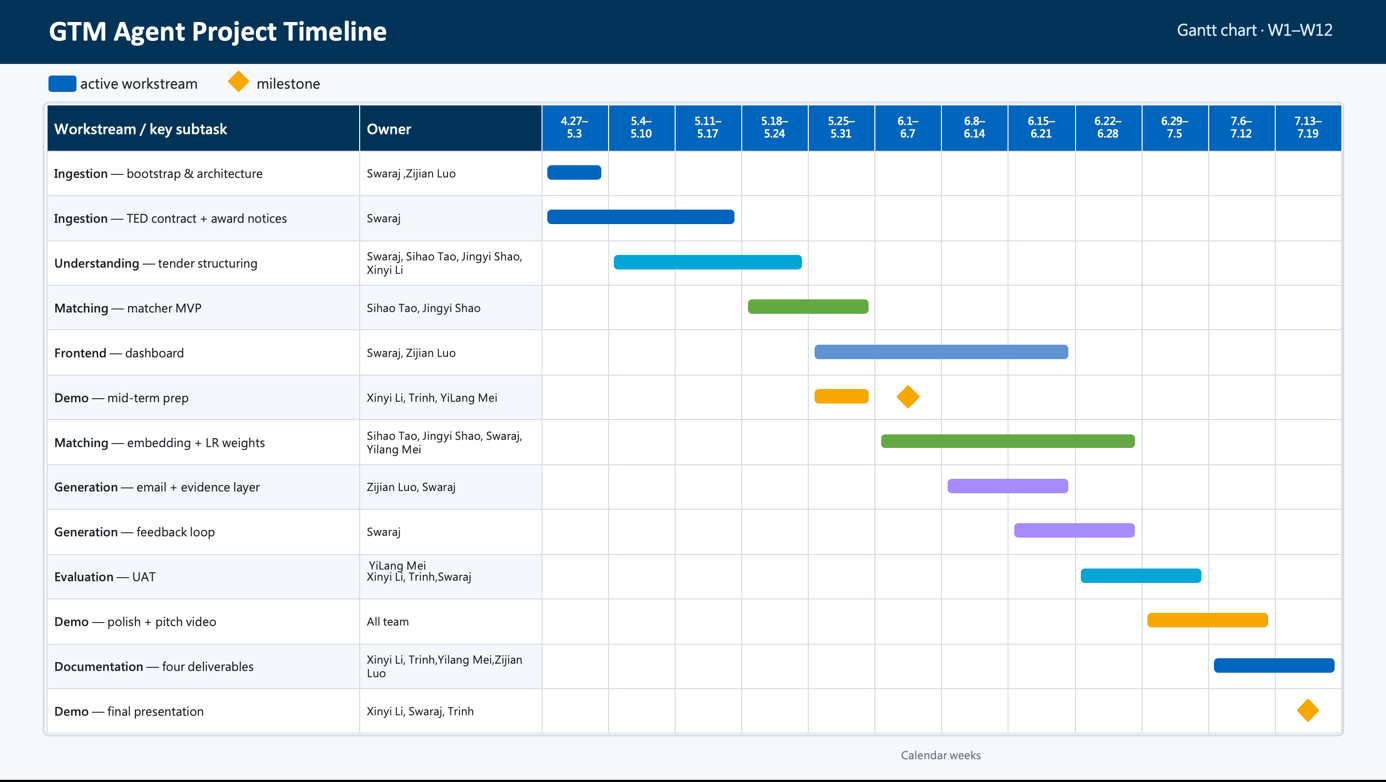
\includegraphics[width=0.98\linewidth]{pm_timeline.png}
\caption[Project timeline]{Project timeline (workstreams and milestones over teaching
weeks W1--W12).\label{fig:timeline}}
\end{figure}

\subsection{Milestones}

The roadmap in Figure~\ref{fig:milestones} groups the same twelve weeks into three
stages. It moves from data ingestion and MVP construction to matching, email, and
retraining features. The final stage covers UAT, documentation, presentation, and
submission.

\begin{figure}[!ht]
\centering
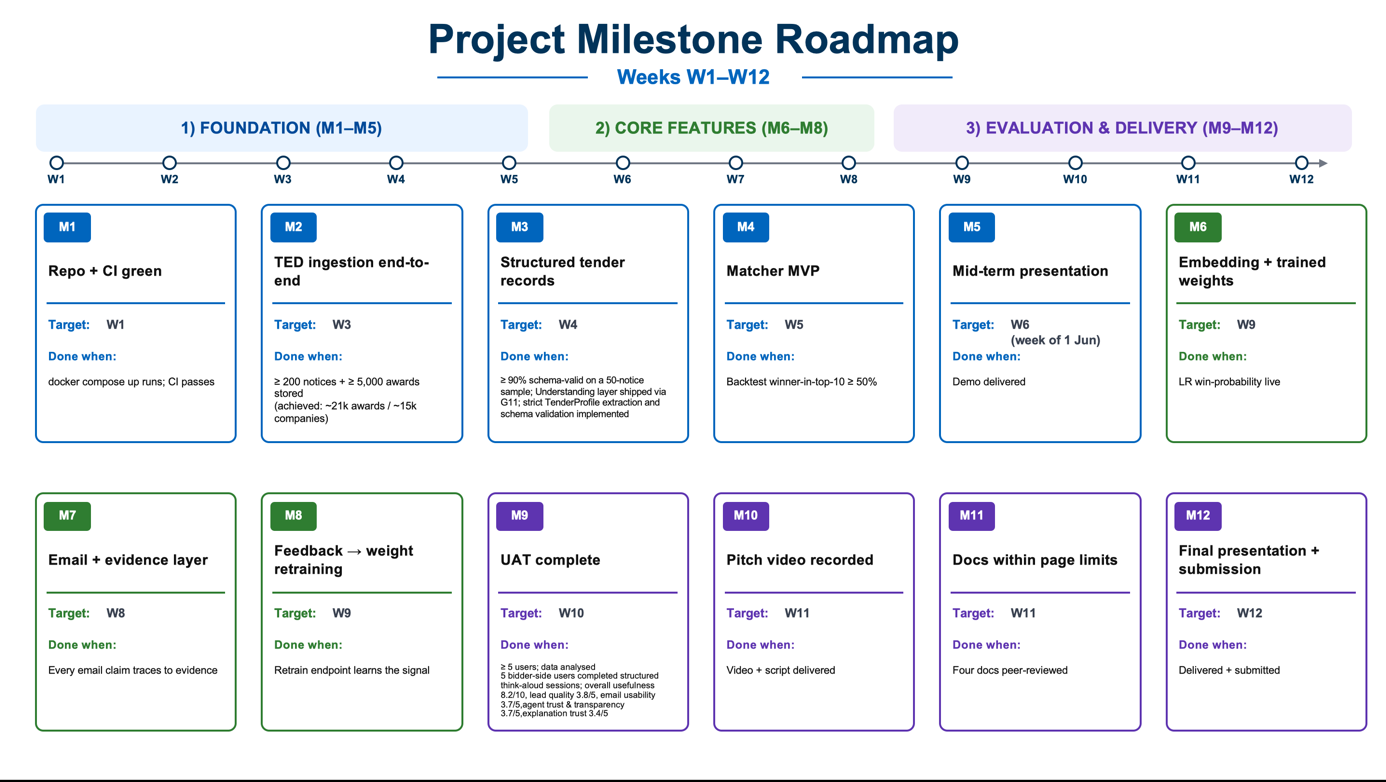
\includegraphics[width=0.98\linewidth]{pm_milestone.png}
\caption[Milestone roadmap]{Milestone roadmap across the three project
stages.\label{fig:milestones}}
\end{figure}

\section{System Architecture}

GTM Agent is organised into seven sub-systems, spanning data ingestion, storage,
matching, evidence-grounded generation, and agent orchestration.
Figure~\ref{fig:architecture} shows how they connect, and the paragraphs below
describe each in turn.

\begin{figure}[!ht]
\centering
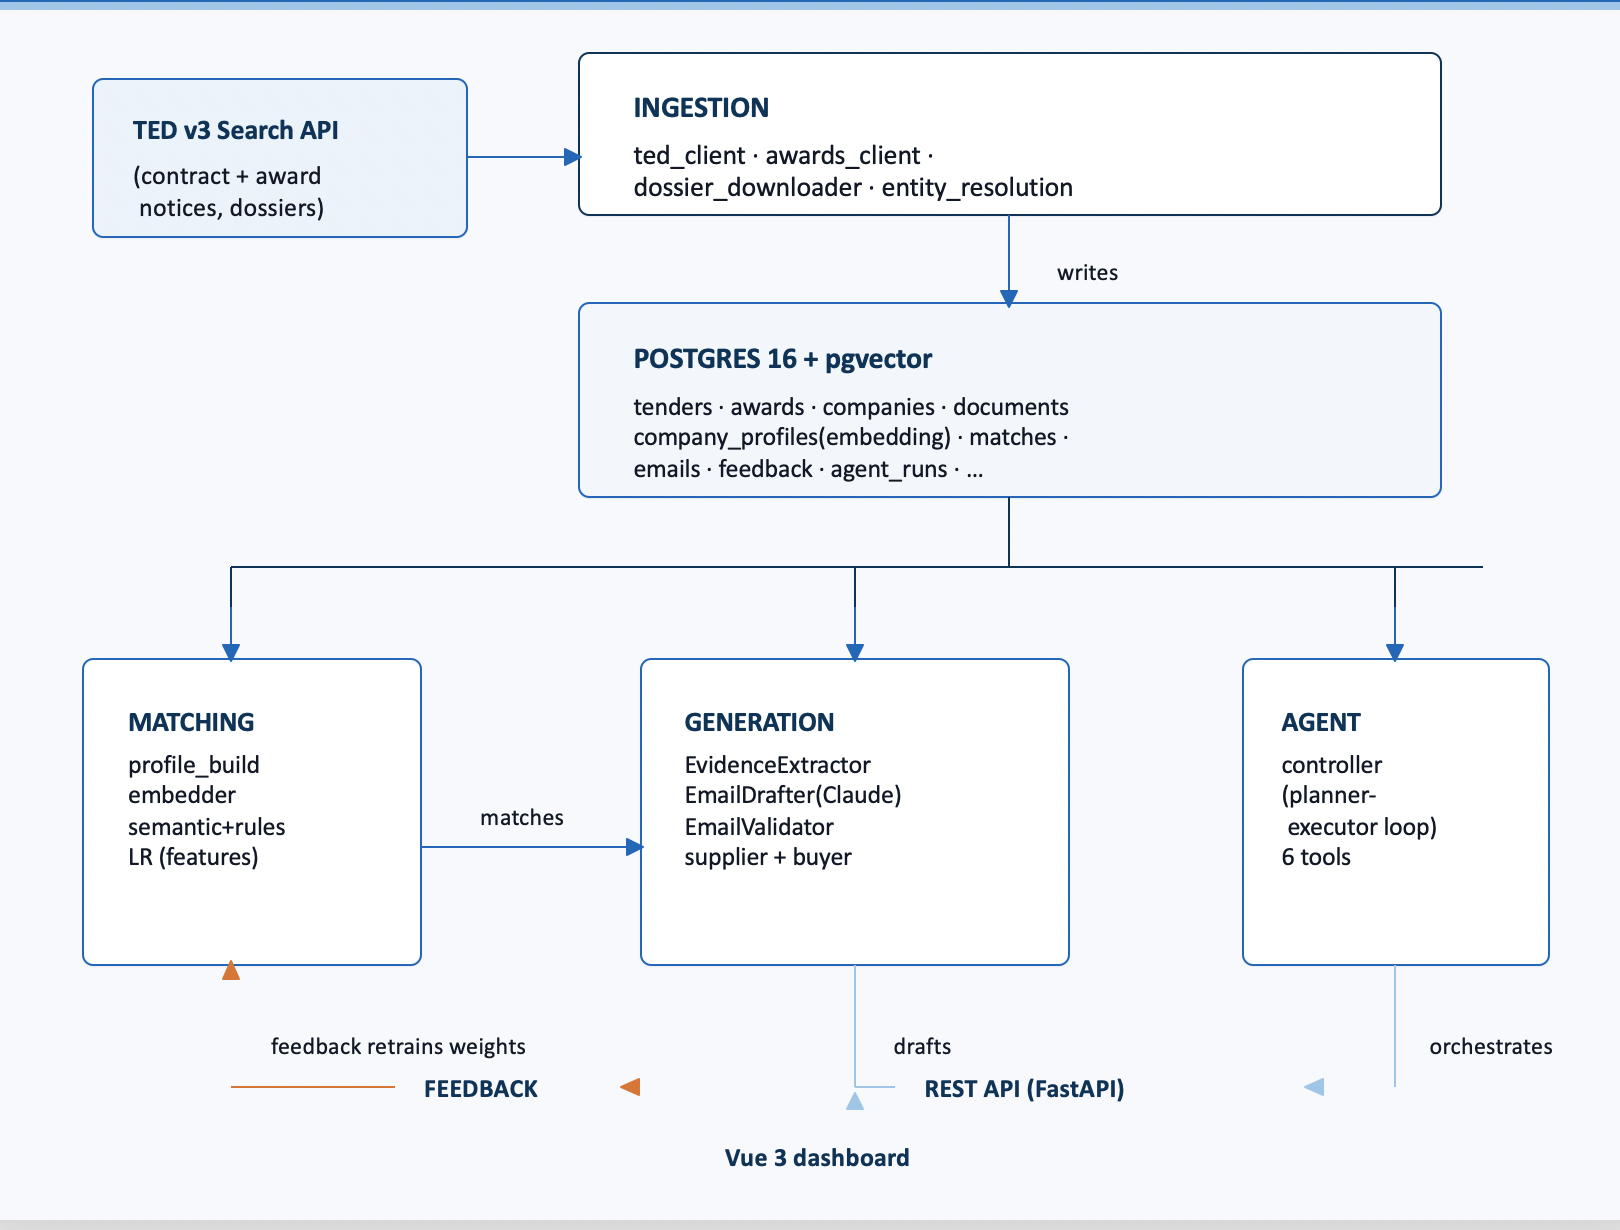
\includegraphics[width=0.90\linewidth]{pm_architecture.png}
\caption[System architecture]{System architecture: ingestion, storage, matching,
generation, and agent.\label{fig:architecture}}
\end{figure}

\subsection{Sub-systems}

\textbf{1. Ingestion.} The module retrieves live Contract Notices and historical
Award Notices through the TED v3 Search API and stores them in PostgreSQL.
Accessible dossier PDFs are downloaded, validated, deduplicated with SHA-256, and
converted to text. Command-line jobs include retry and rate-limit handling to
improve reliability.

\textbf{2. Entity Resolution.} The module standardizes company names by normalizing
capitalization, punctuation, and legal suffixes. It matches firms primarily through
reliable identifiers such as tax IDs and otherwise uses canonical names, while
filtering invalid identifiers to prevent incorrect merges.

\textbf{3. Tender Understanding.} The module converts notice and dossier content
into a structured TenderProfile, covering fields such as budget, deadline, CPV codes,
qualifications, and technical requirements. Outputs follow a strict JSON schema and
are validated through CPV repair, budget checks, and deduplication.

\textbf{4. Matching.} The matching module builds company profiles from historical
awards, including capabilities, embeddings, project scale, and location. It then
filters candidates by CPV, region, budget, and qualifications before using semantic
features and a Logistic Regression model whose output is calibrated to a usable win
probability (Niculescu-Mizil \& Caruana, 2005), implemented in scikit-learn
(Pedregosa et al., 2011).
Sub-scores and explanations show users why each company is ranked.

\textbf{5. Generation.} The system generates supplier outreach emails and buyer
tender digests. An Evidence Extractor supplies verified facts, and Claude drafts the
email under evidence constraints, with a deterministic template as fallback. An Email
Validator rejects unsupported claims, and all drafts require user review before
sending.

\textbf{6. Agent.} The Agent uses Claude's tool-use capability to turn
natural-language goals into executable steps, including data retrieval, matching,
email drafting, and read-only database queries. A planner--executor workflow streams
each step to the interface. For safety, write tools default to dry-run mode, database
access is limited to read-only SELECT queries, and external requests are strictly
bounded.

\textbf{7. API and frontend.} The FastAPI backend provides REST endpoints for
tenders, awards, companies, matches, emails, feedback, and Agent functions, with
automatic OpenAPI documentation. The Vue 3 frontend supports tender browsing,
candidate review, weight adjustment, score explanations, and email approval. Sample
data is used as a fallback when the backend is unavailable.

\subsection{Data model (selected)}
The system stores tenders, awards, companies, profiles, matches, emails, feedback,
and Agent runs in a unified PostgreSQL schema. \texttt{company\_profiles} uses
pgvector to store 384-dimensional embeddings for similarity matching, while a general
embeddings table supports future models. Company master data and capability profiles
are kept separately because they have different sources and update cycles. Full schema
details are documented in \texttt{docs/Database\_Explanation.md}.

\section{Method}

\subsection{Methodological principles}
Three principles shaped every technical decision:

\begin{enumerate}
\tightlist
\item \textbf{Classical ML over LLM where one exists.} The ranking of the matches is
  done by embeddings and logistic regression, not by asking an LLM, giving
  reproducible and explainable scores.
\item \textbf{Open-source, locally-run embedding models.} The most frequent operation
  in the pipeline --- semantic similarity between a tender's requirements and a
  company's portfolio --- runs locally, so there is no per-query API cost.
\item \textbf{Constrain the LLM to extraction and drafting.} The LLM never does
  free-form ranking or makes unverified factual claims. Because fluent but
  unsupported output is a known failure mode of generative models (Ji et al., 2023),
  restricting the model to evidence-backed information is a design constraint rather
  than a stylistic preference.
\end{enumerate}

\subsection{Hybrid matching method}
The core engineering of GTM Agent is its hybrid matching pipeline, which decomposes
the problem into independent layers, each using the right tool
(Table~\ref{tab:layers}).

\begin{table}[!ht]
\centering
\caption[Hybrid matching layers]{Hybrid matching: each layer uses the right
tool.}\label{tab:layers}
\renewcommand{\arraystretch}{1.2}
\begin{tabular}{@{}ll@{}}
\toprule
\textbf{Layer} & \textbf{Tool} \\
\midrule
Structured field extraction & LLM (Claude) \\
Semantic similarity & Open-source sentence embeddings \\
Budget / location / qualification & Deterministic rules \\
Weight fusion & Logistic regression \\
\bottomrule
\end{tabular}
\end{table}

\textbf{1) Hard disqualification.} Claude extracts structured fields from the tender
and company sources but does not rank yet. Before any scoring, a disqualifier removes
clearly ineligible candidates using deterministic filters (blacklisting, geographic
eligibility, company size versus budget tier, or tender-specific exclusions), so the
more expensive scoring steps only run on cleaner shortlists.

\textbf{2) Semantic similarity.} For each surviving candidate, a sentence embedding
model converts each text into a fixed-length vector, positioning semantically related
texts close together and making similarity computable as a cosine distance rather than
as word overlap (Reimers \& Gurevych, 2019). The model used is a distilled MiniLM
(Wang et al., 2020) whose multilingual variant is trained so that a sentence and its
translation land at the same point in the vector space (Reimers \& Gurevych, 2020).
That property is what lets a Czech tender be matched against a German company profile
without a translation step --- necessary for a platform like TED.

\textbf{3) Rule-based checks.} Budget overlap, geographic fit, and CPV qualification
are covered by deterministic sub-scores, because they involve structured data with
unambiguous answers: budget fit (after FX normalisation to EUR), geographic fit
(NUTS regions, Regulation (EC) No 1059/2003), and hierarchical CPV qualification
(an exact 8-digit CPV scores 1.0).

\textbf{4) Logistic-regression weight fusion.} A logistic regression, trained on
historical award notices with the ground truth ``did this company actually win?'',
combines ten features into a calibrated win probability; its coefficients give a
clear per-feature explanation. A feedback loop retrains it on thumbs-up/thumbs-down
pairs, storing a lasting feature snapshot with each feedback row so re-matching never
destroys training data.

\subsection{Prompt Engineering}
GenAI is used in three places, each with a deliberate prompting strategy.

\textbf{Structured field extraction.} A chain-of-thought-style prompt, following the
step-by-step decomposition principle of Wei et al.\ (2022), asks the model to describe
the type of section it is reading, list candidate fields, and produce a JSON fragment
following a strict schema. Only the JSON is processed and
checked; shape failures are rejected. The model is prompted in English while
foreign-language source text is included verbatim, using its multilingual reading
ability without a translation step.

\textbf{Evidence-grounded email drafting.} A two-step pattern: a deterministic
extractor first builds the evidence list (TED ID, CPV codes, deadline, match scores,
company facts); the model then receives only that evidence and is instructed to add no
claim outside it. Output is post-validated, and any unsupported entity or claim flags
the draft for review rather than sending. The prompt also tells the model to match the
tender's language automatically.

\textbf{Agent orchestration.} The agent follows the reason-then-act pattern of Yao
et al.\ (2023): it alternates a short planning step with a tool call and feeds the
tool result back before deciding the next step. A planner--executor system prompt
defines the goal, the tool set (as JSON schemas), and safety constraints (DB-first resolution,
offline-by-default ingest, read-only SQL, \texttt{ask\_user} for ambiguity). Tool
definitions and the system prompt stay stable across turns to benefit from prompt
caching, and messages persist to \texttt{agent\_sessions} so a paused run resumes
exactly where it left off.

\section{Technology Used}

The stack is a Python/FastAPI backend, a PostgreSQL + pgvector database, and a Vue 3
frontend, with open-source models for ranking and Claude for generation and the agent
(Table~\ref{tab:tech}).

{\small\renewcommand{\arraystretch}{1.1}%
\begin{xltabular}{\textwidth}{@{}>{\raggedright\arraybackslash}p{2.5cm} >{\raggedright\arraybackslash}p{4.9cm} >{\raggedright\arraybackslash}X@{}}
\caption[Technology stack]{Technology stack.}\label{tab:tech}\\
\toprule
\textbf{Layer} & \textbf{Technology} & \textbf{Notes}\\
\midrule
\endfirsthead
\toprule
\textbf{Layer} & \textbf{Technology} & \textbf{Notes}\\
\midrule
\endhead
\bottomrule
\endlastfoot
Language / runtime & Python 3.11 & Pinned for dependency compatibility\\
HTTP framework & FastAPI 0.115 & First-class Pydantic v2 + OpenAPI\\
Validation & Pydantic v2 & Strict schema enforcement\\
ORM / migrations & SQLAlchemy 2.0 / Alembic & Typed \texttt{Mapped[]} API\\
Database & PostgreSQL 16 + pgvector & Single schema; vector similarity in-DB\\
HTTP client & httpx (+ truststore) & \texttt{requests} banned by spec\\
PDF text & PyMuPDF & Dossier extraction\\
Embeddings & sentence-transformers: paraphrase-multilingual-MiniLM-L12-v2 (384-d), CPU-only & Multilingual MiniLM; lazy-loaded\\
Classical ML & scikit-learn + joblib & Trained logistic-regression matcher (calibrated win-probability)\\
LLM & Anthropic Claude (\texttt{claude-sonnet-4-6}) & Agent, reflection, email drafting\\
Scheduler & APScheduler (in-process) & Opt-in cron loop (ingest + reflect); runtime on/off/status toggle\\
Frontend & Vue 3 / TypeScript / Vite 5 / Pinia / Tailwind & Three-column dashboard\\
CI & GitHub Actions & pytest · lint+build · migration smoke\\
Containerisation & Docker Compose & db + backend + frontend\\
\end{xltabular}}

\section{Current Progress and Future Plans}

Every planned MVP component is implemented, and the components on the critical path
have been smoke-tested against live TED data; Table~\ref{tab:status} summarises their
status, followed by known limitations and future work.

{\small\renewcommand{\arraystretch}{1.1}%
\begin{xltabular}{\textwidth}{@{}>{\raggedright\arraybackslash}p{5.2cm} >{\raggedright\arraybackslash}X@{}}
\caption[Component status]{Component status.}\label{tab:status}\\
\toprule
\textbf{Component} & \textbf{Status}\\
\midrule
\endfirsthead
\toprule
\textbf{Component} & \textbf{Status}\\
\midrule
\endhead
\bottomrule
\endlastfoot
Repo scaffold, schema, CI & Done\\
TED contract-notice ingestion & Done: CPV-filtered, live-verified\\
Award back-fill + entity resolution & Done: \textasciitilde21k awards / \textasciitilde15k companies cleaned and stored; 24-month back-fill planned\\
Dossier downloader + ingestion CLI & Done (scoped): ingestion-only utility; thin coverage\\
Understanding layer (Claude field extractor) & Done: tender profile persisted; soft fields only\\
Matching (hybrid + trained model) & Done: multilingual embeddings (MiniLM), rules, and a calibrated logistic regression; returns top-N with sub-scores; live-smoked\\
Ranking + explanations & Done: per-supplier sub-scores plus explanation; numbers only from \texttt{query\_db}, live score recalculation runs in the browser with no round-trip\\
Email generation (Claude) & Done: constrained generation only; all evidence validated and grounded; live-verified\\
Feedback capture + retraining & Done: feedback retrains the model\\
Scheduler (opt-in) + reflection loop & Done: reflections stored; runtime on/off/status control\\
Agent (DB-first, streaming, resumable, result actions) & Done: planner--executor loop, max 20 turns, every step streamed live; pauses for user input and resumes from the saved session; live-smoked\\
Ops command console & Done: \texttt{/retrain}, \texttt{/reflect}, \texttt{/schedule}, \texttt{/help}\\
REST API (7 routers) + Vue dashboard (7 views) & Done: browse tenders, open detail pages, inspect recommendations, approve and send email; sample-data fallback\\
ML training dataset export + retrain on 80\% of awards & Done: 16,812 training awards\\
\end{xltabular}}

\textbf{Limitations and future plans.} Company profiles come from award history only,
so the supplier pool is limited to companies that have won a listed EU tender;
per-portal dossier scraping is prepared but not yet built, and the external match
fallback (suggesting and scraping websites when no strong internal match exists) is
out of scope. This fixed supplier pool also explains why the certification
disqualifier, although built and linked to the extraction layer, stays inert in
production: the award data carries no supplier-certification field. Because TED
publishes no supplier email addresses, supplier recipients are website-derived and
marked unverified rather than fabricated, consistent with the rule never to create
information it cannot trace to a source.

Three UAT interface requests remain future work at the presentation layer (a city
field in the detail view, a company-website link in the email and detail views, and
shorter tender titles); they were deferred to focus on the agent work. Match alerts
and competitor analysis are also valuable requests that reuse existing components ---
alerts as a scheduled query over stored matches, competitor analysis as aggregation
over already-ingested award history. Finally, vision-model blueprint parsing, a Neo4j
incumbency knowledge graph, and an embedding ensemble (adding \texttt{all-mpnet-base-v2}
and \texttt{multilingual-e5-large}) are catalogued but not committed.

% The per-chapter reference list was consolidated into the report-wide References
% chapter at the end of the document (chapters/references.tex).
